\documentclass[10pt]{article}

\def\Type{LessonCaelan}
\def\TypeNum{Lesson 12}
\def\TypeTitle{Concavity \& The Second Derivative }
\def\Semester{Fall 2021} %Not Used 
\def\Course{MATH 1190 \& 1210}
\def\Targets{ {\bf\color{RedOrange}A1}, {\bf\color{RedOrange}A2} }

\usepackage{preambleDJ}

%\usepackage{ragged2e}


%%%%%%%%%%%% BEGIN DOCUMENT %%%%%%%%%%%%%%%
%%%%%%%%%%%% BEGIN DOCUMENT %%%%%%%%%%%%%%%
%%%%%%%%%%%% BEGIN DOCUMENT %%%%%%%%%%%%%%%
%%%%%%%%%%%% BEGIN DOCUMENT %%%%%%%%%%%%%%%
%%%%%%%%%%%% BEGIN DOCUMENT %%%%%%%%%%%%%%%



\begin{document}

\pagestyle{otherpages}
\thispagestyle{firstpage}
\vs{.6}

\textbf{Intended Learning Outcomes}
After this lesson, you will be able to 

\begin{itemize}
    \item Describe the meaning of concave up/down graphically and using the second derivative. (\target{A1})
    \item Identify concave up/down intervals and inflection points of a function from given graph or formula. (\target{A1})
    \item Represent concepts such as second derivative, concavity, and inflection points graphically. (\target{A1})
    \item Apply the Second Derivative Test to determine the local extrema of a function graphically and algebraically. (\target{A2})
\end{itemize}

\vspace{-0.5cm}

\hrulefill\\


{\bf\color{blue} Warm-up exercise 1.} Describe the relationship between a function $f$, tangent lines, $f^{\prime\prime}$ and ``bendiness" (an informal description of how $f$ is bending).\\



\fbox{
\begin{minipage}{0.95\textwidth}
\mpageT{.55}{.45}{
{\em Concave up} for $x$ on an interval $I$:
\itemI{
\item ``Bendiness":
\item Tangent lines:
\item Derivative $f^{\prime}(x)$ is
\item $\ds f^{\prime\prime}(x)=\frac{d}{dx}[f^{\prime}(x))]$
}
}{
%
\,\hfill 
\includegraphics[width=0.4\textwidth]{images/concavity(2).PNG} \hfill 
\includegraphics[width=0.4\textwidth]{images/concavity(3).PNG} \hfill\,
}
\end{minipage}
}\\[0.1in]
%
\fbox{
\begin{minipage}{0.95\textwidth}
\mpageT{.55}{.45}{
{\em Concave down}  for $x$ on an interval $I$:
\itemI{
\item ``Bendiness":
\item Tangent lines:
\item Derivative $f^{\prime}(x)$ is
\item $\ds f^{\prime\prime}(x)=\frac{d}{dx}[f^{\prime}(x))]$
}
}{
\,\hfill 
\includegraphics[width=0.4\textwidth]{images/concavity(1).PNG} \hfill 
\includegraphics[width=0.4\textwidth]{images/concavity(4).PNG} \hfill\,
}
\end{minipage}
}\\[0.1in]
%
\fbox{
\begin{minipage}{0.95\textwidth}
\mpageT{.55}{.45}{
{\em Inflection point}  at $x$:
\itemI{
\item Concavity
\item $f^{\prime\prime}(x)=$
}
}{
\,\hfill 
\includegraphics[width=0.4\textwidth]{images/inflectionpoint.PNG} \hfill\,
}
\end{minipage}
}\\

\newpage
{\bf\color{blue}Warm-up exercise 2.}\ltrm{\color{RedOrange}A1}Identify which intervals $f$ would be {\it concave down} and inflection points if...\\\mpageTth{.33}{.33}{.33}[\hs{.1}][\hs{.1}]{
\enumA{\item the curve pictured below were the graph of $f$?}\vs{-.2}
\begin{center}
    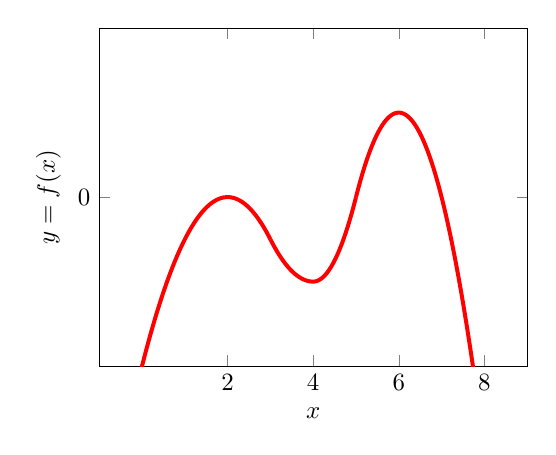
\begin{tikzpicture}[scale=.9]
          \begin{axis}[
            xlabel={$x$},
            ylabel={$y=f(x)$},
            %grid = major,
            xtick       = {2,4,6,8},
            xticklabels = {$2$,$4$,$6$,$8$},
            ytick       = {0},
            yticklabels = {$0$},
            samples     = 320,
            domain      = -1:9,
            restrict y to domain=-40:40,
            xmin = -1, xmax = 9,
            ymin = -4, ymax = 4,
            height=2.5in, width=3in
          ]
          \addplot[domain=-1:3, ultra thick, red] {-(x-2)^2};
          \addplot[domain=3:4, ultra thick, red] {(x-4)^2-2};
          \addplot[domain=4:5, ultra thick, red] {2*(x-4)^2-2};
          \addplot[domain=5:9, ultra thick, red] {-2*(x-6)^2+2};
          %
        \end{axis}
    \end{tikzpicture}
\end{center}
}{
\enumA{\setItemnumber{2}\item the curve pictured below were the graph of $f'$?}\vs{-.2}
\begin{center}
    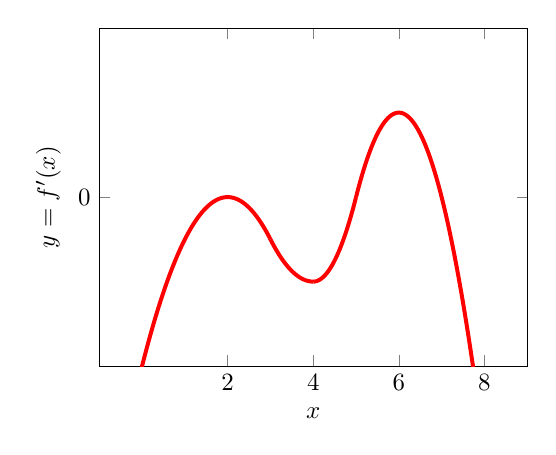
\begin{tikzpicture}[scale=.9]
          \begin{axis}[
            xlabel={$x$},
            ylabel={$y=f^{\prime}(x)$},
            %grid = major,
            xtick       = {2,4,6,8},
            xticklabels = {$2$,$4$,$6$,$8$},
            ytick       = {0},
            yticklabels = {$0$},
            samples     = 320,
            domain      = -1:9,
            restrict y to domain=-40:40,
            xmin = -1, xmax = 9,
            ymin = -4, ymax = 4,
            height=2.5in, width=3in
          ]
          \addplot[domain=-1:3, ultra thick, red] {-(x-2)^2};
          \addplot[domain=3:4, ultra thick, red] {(x-4)^2-2};
          \addplot[domain=4:5, ultra thick, red] {2*(x-4)^2-2};
          \addplot[domain=5:9, ultra thick, red] {-2*(x-6)^2+2};
          %
        \end{axis}
    \end{tikzpicture}
\end{center}
}{
\enumA{\setItemnumber{3}\item the curve pictured below were the graph of $f''$?}\vs{-.2}
\begin{center}
    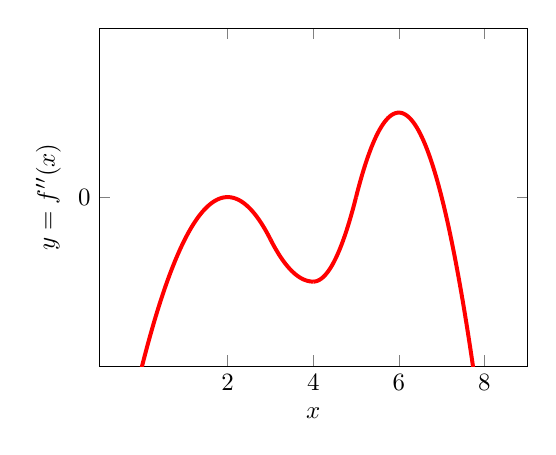
\begin{tikzpicture}[scale=.9]
          \begin{axis}[
            xlabel={$x$},
            ylabel={$y=f^{\prime \prime}(x)$},
            %grid = major,
            xtick       = {2,4,6,8},
            xticklabels = {$2$,$4$,$6$,$8$},
            ytick       = {0},
            yticklabels = {$0$},
            samples     = 320,
            domain      = -1:9,
            restrict y to domain=-40:40,
            xmin = -1, xmax = 9,
            ymin = -4, ymax = 4,
            height=2.5in, width=3in
          ]
          \addplot[domain=-1:3, ultra thick, red] {-(x-2)^2};
          \addplot[domain=3:4, ultra thick, red] {(x-4)^2-2};
          \addplot[domain=4:5, ultra thick, red] {2*(x-4)^2-2};
          \addplot[domain=5:9, ultra thick, red] {-2*(x-6)^2+2};
          %
        \end{axis}
    \end{tikzpicture}
\end{center}
}


\vs{1}

{\bf\color{blue}Mini-lecture.}  Last time, we located local extrema using the First Derivative Test. Today,  we {\it locate local extrema using the Second Derivative Test}.\\
\mpageT{.5}{.5}{\centering
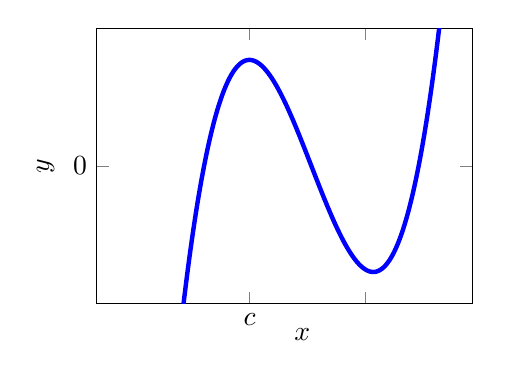
\begin{tikzpicture}[scale=1]
          \begin{axis}[
            xlabel={$x$},
            xlabel style={anchor=west},
            ylabel={$y$}, 
            ylabel style={anchor=south},
            %grid = major,
            xtick       = {1.85,4,6,8},
            xticklabels = {$c$,,,},
            ytick       = {0},
            yticklabels = {$0$},
            samples     = 320,
            domain      = -1:6,
            restrict y to domain=-40:40,
            xmin = -1, xmax = 6,
            ymin = -4, ymax = 4,
            height=2in, width=2.5in
          ]
          % old version of the curve
          %
          %\addplot[domain=-1:9, purple, ultra thick, mark=none] {-1/10*(x-1)*(x-4)^2*(x-7)};
          %
          %new version of the curve in pieces
          %
          \addplot[domain=0:6, ultra thick, blue] {((x-1)*(x-3)*(x-5)};
          %
        \end{axis}
    \end{tikzpicture}
\captionof*{figure}{\bf Local Maximum}
}{\centering
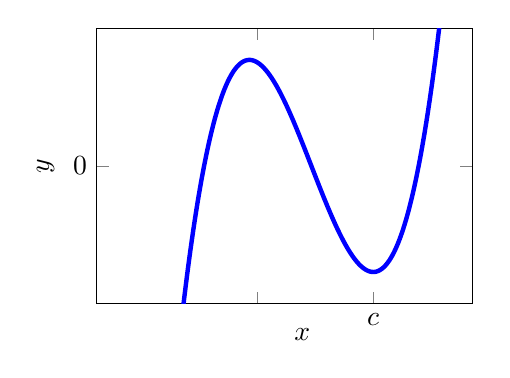
\begin{tikzpicture}[scale=1]
          \begin{axis}[
            xlabel={$x$},
            xlabel style={anchor=west},
            ylabel={$y$}, 
            ylabel style={anchor=south},
            %grid = major,
            xtick       = {2,4.15,6,8},
            xticklabels = {,$c$,,},
            ytick       = {0},
            yticklabels = {$0$},
            samples     = 320,
            domain      = -1:6,
            restrict y to domain=-40:40,
            xmin = -1, xmax = 6,
            ymin = -4, ymax = 4,
            height=2in, width=2.5in
          ]
          % old version of the curve
          %
          %\addplot[domain=-1:9, purple, ultra thick, mark=none] {-1/10*(x-1)*(x-4)^2*(x-7)};
          %
          %new version of the curve in pieces
          %
          \addplot[domain=0:6, ultra thick, blue] {((x-1)*(x-3)*(x-5)};
          %
        \end{axis}
    \end{tikzpicture}
\captionof*{figure}{\bf Local Minimum}
}
\vs{1}

\important{Second Derivative Test}
{
Suppose $f''$ is continuous near a critical number $x=c$.
\enumA{
\item If \hfill  Local Maximum at $x=c$\\
\item  If \hfill  Local Minimum at $x=c$\\
\item If \hfill Second Derivative Test is inconclusive.\\
}
}
\newpage
{\example} Let $g(x)=\dfrac{1}{x^2+1}$.  $g^{\prime}(x)=\dfrac{-2x}{(x^2+1)^2}$ and $g^{\prime\prime}(x)=\dfrac{6x^2-2}{(x^2+1)^3}$.
\enumA{
\item\ltrm{\color{RedOrange}A1} Find the intervals on which $g$ is concave up and on which $g$ is concave down. Does the graph of $g$ have any inflection points? If so, then specify their $x$-coordinates. If not, then explain.
    \vfill
    \vfill

\item\ltrm{\color{RedOrange}A2} Recall that the only critical number of $g$ was $x=0$, with $g'(0)=0$. What does the Second Derivative Test tell us about the behavior of $g$ at its critical numbers?
    \vfill
    
}

\newpage

{\exercise} Let $f(x)=\dfrac{x}{x^2+1}$.
\enumA{
\item\ltrm{\color{RedOrange}A1} Find the critical numbers of $f$. {\em Hint}: We found the first derivative of this function in Lesson $11$.

    \vfill

\item\ltrm{\color{RedOrange}A1} Given $f''(x)=\dfrac{2x(x+\sqrt3)(x-\sqrt3)}{(x^2+1)^3}$, find the intervals of $x$-values on which $f$ is concave up and on which $f$ is concave down.

    \vfill
    \vfill

\item\ltrm{\color{RedOrange}A1} What are the $x$-coordinates of the inflection points of the graph of $f$? If there are multiple such values, then separate them with commas.
{\Large
x=\unline{1}{}{.25}
}
    \vfill
\item\ltrm{\color{RedOrange}A2} What does the Second Derivative Test tell you about the behavior of $f$ at its critical numbers? Explicitly use the Second Derivative Test in your response.

    \vfill

    
}

%%%%%%%%%
\newpage%
%%%%%%%%%

\paragraph*{Note:} The following problem is based on a problem appearing on an exam during the Fall 2023 semester.\\\\
{\bf\color{blue}Exam Practice 1.}\ltrm{\color{RedOrange}A1} What would the $x$-coordinates of inflection points on the graph of $f$ be if....  \\
Justify your answers using relevant definitions or properties from the first page of this activity.

\mpageT{.5}{.5}{
\enumA{\item the curve pictured to the right is the graph of $f$?}
}{
\begin{flushright}
    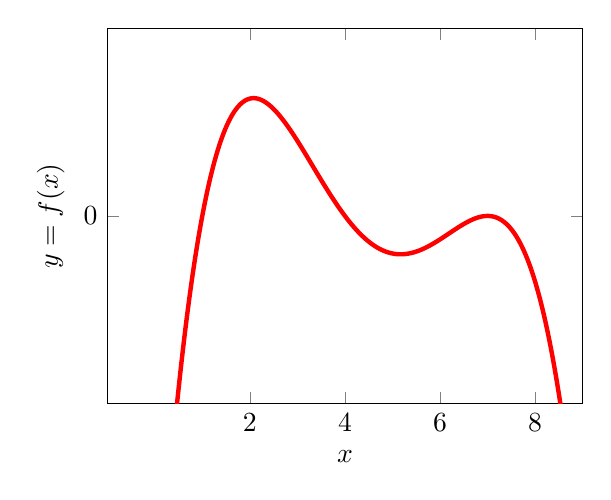
\begin{tikzpicture}[scale=1]
          \begin{axis}[
            xlabel={$x$},
		ylabel={$y=f(x)$},
            %grid = major,
            xtick       = {2,4,6,8},
            xticklabels = {$2$,$4$,$6$,$8$},
            ytick       = {0},
            yticklabels = {$0$},
            samples     = 320,
            domain      = -1:9,
            restrict y to domain=-40:40,
            xmin = -1, xmax = 9,
            ymin = -4, ymax = 4,
            height=2.5in, width=3in
          ]
          % old version of the curve
          %
          %\addplot[domain=-1:9, purple, ultra thick, mark=none] {-1/10*(x-1)*(x-4)^2*(x-7)};
          %
          %new version of the curve in pieces
          %
%          \addplot[domain=-1:3, ultra thick, red] {-(x-2)^2};
%          \addplot[domain=3:4, ultra thick, red] {(x-4)^2-2};
%          \addplot[domain=4:5, ultra thick, red] {2*(x-4)^2-2};
%          \addplot[domain=5:9, ultra thick, red] {-2*(x-6)^2+2};
          %
          %even newer
            \addplot[domain=-1:9, purple, ultra thick, red, mark=none] {-1/20*(x-1)*(x-4)*(x-7)^2};
        \end{axis}
    \end{tikzpicture}
\end{flushright}
}
\vfill

\mpageT{.5}{.5}{
\enumA{\setItemnumber{2} \item the curve pictured to the right is the graph of $f'$?}
}{
\begin{flushright}
    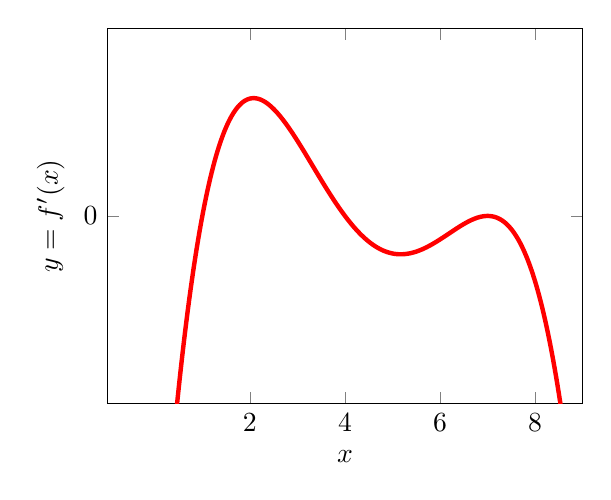
\begin{tikzpicture}[scale=1]
          \begin{axis}[
            xlabel={$x$},
		ylabel={$y=f^{\prime}(x)$},
            %grid = major,
            xtick       = {2,4,6,8},
            xticklabels = {$2$,$4$,$6$,$8$},
            ytick       = {0},
            yticklabels = {$0$},
            samples     = 320,
            domain      = -1:9,
            restrict y to domain=-40:40,
            xmin = -1, xmax = 9,
            ymin = -4, ymax = 4,
            height=2.5in, width=3in
          ]
          % old version of the curve
          %
          %\addplot[domain=-1:9, purple, ultra thick, mark=none] {-1/10*(x-1)*(x-4)^2*(x-7)};
          %
          %new version of the curve in pieces
          %
%          \addplot[domain=-1:3, ultra thick, red] {-(x-2)^2};
%          \addplot[domain=3:4, ultra thick, red] {(x-4)^2-2};
%          \addplot[domain=4:5, ultra thick, red] {2*(x-4)^2-2};
%          \addplot[domain=5:9, ultra thick, red] {-2*(x-6)^2+2};
          %
            %even newer
            \addplot[domain=-1:9, purple, ultra thick, red, mark=none] {-1/20*(x-1)*(x-4)*(x-7)^2};
        \end{axis}
    \end{tikzpicture}
\end{flushright}
}
\vfill

 \mpageT{.5}{.5}{
\enumA{\setItemnumber{3} \item the curve pictured to the right is the graph of $f''$?}
}{
\begin{flushright}
    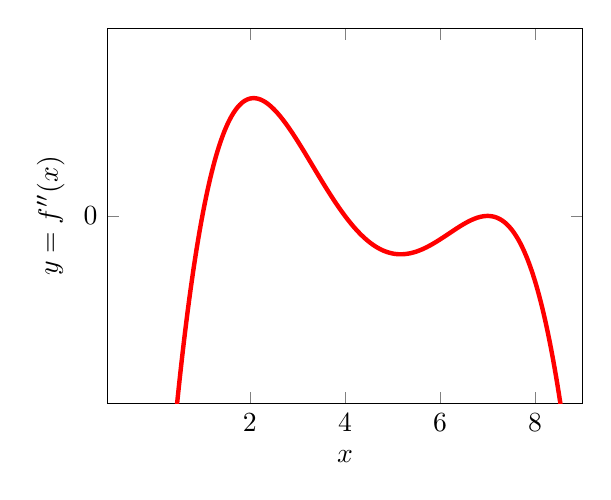
\begin{tikzpicture}[scale=1]
          \begin{axis}[
            xlabel={$x$},
		ylabel={$y=f^{\prime\prime}(x)$},
            %grid = major,
            xtick       = {2,4,6,8},
            xticklabels = {$2$,$4$,$6$,$8$},
            ytick       = {0},
            yticklabels = {$0$},
            samples     = 320,
            domain      = -1:9,
            restrict y to domain=-40:40,
            xmin = -1, xmax = 9,
            ymin = -4, ymax = 4,
            height=2.5in, width=3in
          ]
          % old version of the curve
          %
          %\addplot[domain=-1:9, purple, ultra thick, mark=none] {-1/10*(x-1)*(x-4)^2*(x-7)};
          %
          %new version of the curve in pieces
          %
%          \addplot[domain=-1:3, ultra thick, red] {-(x-2)^2};
%          \addplot[domain=3:4, ultra thick, red] {(x-4)^2-2};
%          \addplot[domain=4:5, ultra thick, red] {2*(x-4)^2-2};
%          \addplot[domain=5:9, ultra thick, red] {-2*(x-6)^2+2};
          %
            %even newer
            \addplot[domain=-1:9, purple, ultra thick, red, mark=none] {-1/20*(x-1)*(x-4)*(x-7)^2};
        \end{axis}
    \end{tikzpicture}
\end{flushright}
}
\vfill



%%%%%%%%%
\newpage%
%%%%%%%%%

{\bf\color{blue} Extra Practice 1.} Let $g(x)=x^{2/3}(x+2)$. You may take as given that $g'(x)=\dfrac{5x+4}{3\sqrt[3]{x}}$ and $g''(x)=\dfrac{2(5x-2)}{9x^{4/3}}$.
\enumA{
\item\ltrm{\color{RedOrange}A1} Find the intervals where the graph of $g$ is concave up and concave down.
\vfill



\item\ltrm{\color{RedOrange}A1} Specify the $x$-coordinates of any inflection points on the graph of $g$.
\vfill



\item\ltrm{\color{RedOrange}A2} What does the Second Derivative Test tell us about the behavior of $g$ at its critical numbers?
\vfill
}


\end{document}
